\chapter{概论}
深度强化学习(deep reinforcement learning:DRL)结合了深度神经网络和强化学习的优势,可以解决机器在复杂的高维度状态空间中的感知和决策问题。在游戏领域,无人驾驶,推荐系统,机器人等领域,深度强化学习已经取得了突破性进展\cite{唐振韬2017深度强化学习进展,赵冬斌2016深度强化学习综述:兼论计算机围棋的发展,Li2017Deep,arulkumaran2017brief}。强化学习属于无监督学习,强化学习与其他机器学习任务的显著区别在于:没有预先给出训练数据,而是要通过与环境的交互产生;在环境中执行一个动作,没有关于这个动作的好坏标记,而只有在交互一段时间后才能得知累积奖励,从而推断出之前动作的好坏。通常情况下马尔科夫决策过程(Markov Decision Process,MDP)被用来描述强化学习所需要进行的一系列任务,具体而言:机器将会处于一个没有人为干扰的客观环境中,机器当前的状态就是当前机器对环境里的感知(例如声音,图像等),机器处于环境中的每一个状态时可以选择执行多个动作中的一个,当机器选择执行完成某一个动作的时候,当前环境会按照某个概率转换成另一个状态;与此同时当前环境会根据背后已经规定好的规则反馈给机器一些有用的信息(例如评价这个机器当前做得好不好)。总的来说,强化学习主要包含:环境的状态、机器可以选择的动作、机器从当前状态转移到下一个状态的转移概率、环境在机器执行动作后反馈的奖赏函数四个要素\cite{2011机器学习及其应用}。

在人工智能这个领域,衡量智能的关键指标是机器的感知和决策能力。伴随着近几年强化学习和深度学习的发展,直接根据原始数据来提取的高水平特征并进行感知决策不再困难\cite{唐振韬2017深度强化学习进展}。深度强化学习在最近短短几年的时间里取得了很多进展,同时也在机器学习这个领域中得到了很多学者的关注。传统强化学习的局限性在于动作和样本的空间都很小,而且一般是离散的场景。在实际的任务中往往要求高维的状态空间和连续的空间动作,传统强化学习无法处理这样非常复杂的场景。伴随着近几年深度学习的研究进步,深度学习在处理高维度输入具有强大的能力且能产生优异的效果,如果可以将深度学习用来处理传统强化学习的输入,将深度学习神经网络与传统强化学习相结合,那么既可以拥有深度学习强大的环境理解能力,也可以拥有强化学习优秀的决策能力。

强化学习对机器所处不同状态优秀的决策能力和深度学习强大的环境理解感知能力结合而成的深度强化学习成为人工智能领域一个新的研究热点,通过端到端(end-to-end)的学习方式,可以实现数据的原始输入到输出的的直接控制\cite{唐振韬2017深度强化学习进展}。许多需要高维度原始输入数据的决策控制任务,如声音、图像的高维度输入、机器人的控制等,在这些复杂的任务中深度强化学习已经取得了实质性的突破。

在本课题中,我们将使用深度强化学习的经典算法DQN及其三大改进算法控制经典游戏超级玛丽运动到距离起点更远的距离。主要的难点在于超级玛丽相比于其他Atari游戏,控制更加困难,逻辑更加复杂,游戏中还会遇到NPC(非玩家控制角色)与Agent的交互。

本论文由以下几个部分构成:第一章是针对深度强化学习的发展以及研究现状的概论;第二章重点讲解DQN算法原理,以及DQN算法三个重大改进的原理;第三章是整个课题的实验实施设计,包括游戏控制环境,逻辑流程,神经网络的整体结构,控制算法的工作流程以及游戏控制的关键难点;第四章是对实验结果的分析报告,包括实验结果的数据情况、结论,以及分析未来需要进行的改进措施;第五章是对本次课题做的总结,分析存在的问题,实验效果,改进方向等。
\begin{figure}
  \centering
  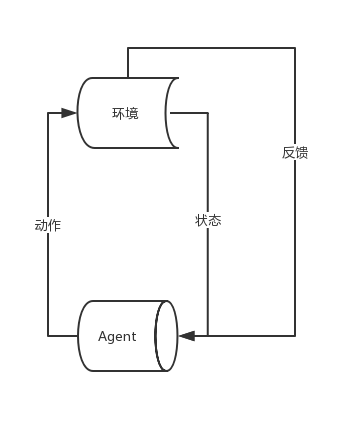
\includegraphics[scale=0.5]{static/RL.png}
  \caption{强化学习示意图}
\end{figure}
\cleardoublepage

\section{深度强化学习的发展概况
}
\subsection{传统强化学习}
传统强化学习主要分为基于价值的Q-learning\cite{Mnih2013Playing},和基于策略的Sarsa。\begin{equation}\label{eq:DQN}
  Q\left(s_{t}, a_{t}\right) \leftarrow Q\left(s_{t}, a_{t}\right)+\alpha\left[r_{t+1}+\gamma \max _{a} Q\left(s_{t+1}, a\right)-Q\left(s_{t}, a_{t}\right)\right]  
\end{equation}

Q-learning(\ref{eq:DQN})主要通过一张Q-table作为输入状态与输出动作价值的估计,通过Q-table来进行更新。
Sarsa(\ref{eq:Sarsa})是一种在线学习的算法,Q-learning是一种离线学习算法。Sarsa选取的是一种保守的策略,他在更新Q值的时候已经为未来规划好了动作,对死亡和错误比较敏感;Q-learning算法相比较而言更加大胆,Q-learing在更新的时候选取的是最大Q值的方向,对死亡和错误不敏感。
\begin{equation}\label{eq:Sarsa}
  Q\left(s_{t}, a_{t}\right) \leftarrow Q\left(s_{t}, a_{t}\right)+\alpha\left[r_{t+1}+\gamma Q\left(s_{t+1}, a_{t+1}\right)-Q\left(s_{t}, a_{t}\right)\right]
\end{equation}

\subsection{深度学习的兴起}
\begin{figure}[!htp]
  \centering
  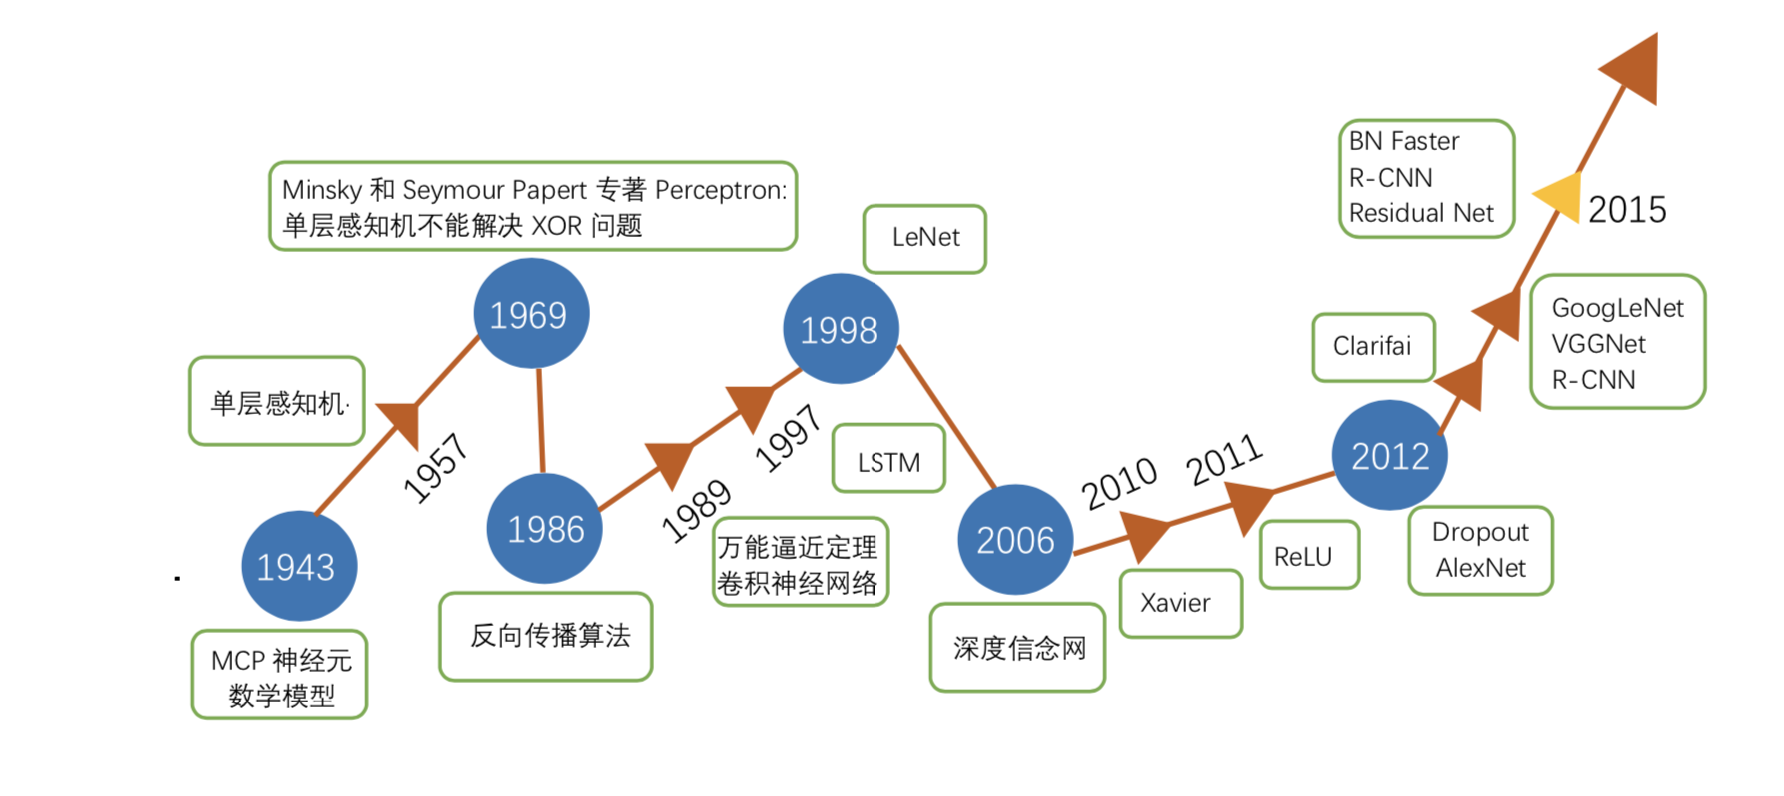
\includegraphics[scale=0.5]{static/develop.png}
  \caption{深度学习的发展}
\end{figure}
深度学习(Deep Learning:DL)这个概念在很早之前就已经提出,但是在深度学习的发展经历过数次的高潮,也经历过数次低谷,在最近几年开始重新成为热门研究话题。MCP人工神经元模型早在1943年就被提出,希望能够通过计算机来模拟人类的神经元处理输入信号的反应过程。MCP模型将神经元简化为:输入信号线性加权,求和操作,非线性函数激活(阈值法)输出。Minsky在1969年经过深入的研究,得出感知器在本质上是线性模型,只能处理线性分类问题,无法处理非线性问题\cite{Rosenblatt1958The}。在证明了感知器存在的这种局限性之后,神经网络的发展迎来持续数十年寒冬时期。适用于多层感知器(MLP)的BP(反向传播)算法\cite{rumelhart1988learning}于1989年被提出,也被称为BP神经网络。BP神经网络引入了一种特殊的激活函数Sigmoid激活函数,通过这种函数可以对神经网络进行非线性映射,有了非线性映射关系,非线性分类问题(如XOR异或问题)得到了有效解决,同时BP算法使得神经网络能进行有效地更新学习。在1989年LeCun发明了卷积神经网络Le-Net\cite{lecun1998gradient},并将其用于数字识别,虽然取得了较好的效果,但是在当时并没有引起足够的注意。1991年,BP算法被指出存在梯度爆炸或梯度消失问题,由于Sigmoid函数的饱和特性,在深层神经网络误差梯度后向传递的过程中,后层梯度以乘性方式叠加到前层,误差梯度传到前层时几乎为0,因此无法对前层进行有效的学习。2006年是深度学习元年,Hinton提出了深层网络训练中梯度消失问题的解决方案。通过无监督预训练对权值进行初始化和有监督训练微调\cite{hinton2006fast}这两种方式,能够有效解决深层神经网络训练中出现的梯度爆炸或者梯度消失的问题。2012年Hinton使用AlexNet\cite{krizhevsky2012imagenet}的神经网络结构参加ImageNet比赛,一举夺得冠军,并且大幅超越第二名传统机器学习SVM的正确率。在随后的几年中,通过ImageNet图像识别比赛。随着深度学习研究的发展以及硬件计算能力的提升,深度学习在其他领域也表现出强大的生命力。在ImageNet之后深度学习受到了广泛的关注,越来越多的深度学习研究开展,并且在不同的领域展现出其强大的学习能力。其中卷积神经网络(CNN)的提出,极大的促进了计算机在图像处理方面的发展,特别是图像识别已经达到远远超越人类的水平。
\subsection{深度强化学习发展}
由于深度学习在人工智能领域的大放异彩,2013年DeepMind的DQN\cite{Mnih2013Playing}(Deep Q-Network:深度Q网络)是将深度学习和强化学习成功结合的开端。DQN算法用一个神经网络代表价值函数,根据传统强化学习中的Q-Learning算法为神经网络提供目标值,通过网络不断更新直至收敛来学习感知和决策的能力。DQN在Atari上取得超越之前所有算法,并在其中6个游戏中取得了超越人类的成绩。DQN算法用到了两个关键技术:
\begin{enumerate*}
  \item 使用经验库打破样本间关联性;
  \item 使用固定目标网络使得训练的稳定性和收敛性更好。
\end{enumerate*}

DQN算法是整个深度强化学习研究的开山之作,引起了许多研究团队和学者的关注。DQN算法的主要改进如下表展示,其中double DQN\cite{van2016deep}、优先级经验回放(Priorized Experience Replay)DQN\cite{schaul2015prioritized}、竞争架构(Dueling-Net)DQN\cite{wang2015dueling}是DQN算法最为代表性的三大改进。在DQN算法取得很大成功之后,受到了越来越多的关注,之后有更多算法的提出,深度强化学习不断地涌现强大的生命力。
\begin{table}
  \centering
  \caption{DQN改进算法\cite{唐振韬2017深度强化学习进展}}
  \begin{tabular}{@{}llr@{}} \toprule
    年份 & 研究单位 & 算法 \\ \hline
    2015 & DeepMind & DQN \\ \hline
    2015 & DeepMind & 分布式DQN\cite{nair2015massively} \\ \hline
    2016 & DeepMind & double DQN\cite{van2016deep} \\ \hline
    2016 & DeepMind & 优先级经验回放 DQN\cite{schaul2015prioritized} \\ \hline
    2016 & DeepMind & dueling DQN\cite{wang2015dueling} \\ \hline
    2016 & Standford \& DeepMind & 引导 DQN\cite{osband2016deep} \\ \hline
    2016 & DeepMind & 异步 DQN\cite{mnih2016asynchronous} \\ \hline
    2017 & Technion & 平均 DQN \\ \hline
    2017 & Illinois Urbana-Champaign & 约束优化 DQN \\ \hline
    2017 & DeepMind & 分类 DQN \\ \hline
    2017 & DeepMind & 噪声 DQN \\ \hline
    2017 & DeepMind & Rainbow \\ \hline
  \end{tabular}
\end{table}
\section{深度强化学习研究现状}
深度强化学习的目前研究主要分为:
\begin{enumerate*}
  \item 基于价值(value based);
  \item 基于策略(policy based);
  \item 基于价值和基于策略结合的Actor-Critic算法。
\end{enumerate*}
\subsection{基于价值}
DQN是多层卷积神经网络,其输出给定状态s和网络参数$\theta$的动作值向量。它是从$R_n$到$R_m$的函数,其中n是状态空间的维度,m是动作空间的维度。 DQN算法的三个关键要素是体验重放,固定目标Q网络,以及限制奖励范围。体验重播解决了之前提出的奖励通常是延时的问题,它有助于打破数据的相关性,并从过去的所有经验中学习,存储一组最近的转换过程以用于某些预定步骤并随机均匀地采样以更新网络。
\subsection{基于策略}
基于价值的强化学习算法的基本思想是根据当前的状态,计算采取每个动作的价值,然后根据价值贪心的选择动作。策略梯度(Policy Gradient)\cite{sutton2000policy}则省略了计算每个动作的价值,而是直接根据当前的状态来选择来进行决策的算法。

策略梯度的核心思想是更新参数时有以下考虑:如果当前回合选择某一动作,那么下一回合选择执行该动作的概率大一些。执行动作完成之后再看环境的反馈,如果反馈是正的,那么就会增加执行这个动作的概率,如果反馈是负的,就会减小执行这个动作的概率。
\subsection{Actor-Critic}
Actor-Critic\cite{Barto1998Reinforcement}是将基于价值(比如DQN)和基于策略(比如Policy Gradient)两类强化学习结合起来。因此Actor-Critic分为两个部分:Actor(基于策略)和Critic(基于价值)。为了介绍这类算法,接下来举一个玩游戏的例子:

Actor(玩家):为了使这个游戏得到尽量高的分数reward(奖励),需要实现一个函数:输入状态(state,如当前的游戏画面),输出动作(action,如上下左右跳跃等)。可以采用神经网络来近似这个函数。剩下的任务就是如何训练神经网络,让它的表现更好(获得得更高的reward)。这个网络就被称为Actor。

Critic(评委):为了训练Actor,需要知道Actor的表现到底怎么样,根据表现来决定对神经网络参数的调整。这就要用到强化学习中的“Q-value(Q价值)”。Q-value也是一个未知的函数,也可以用神经网络来近似。这个网络被称为critic。

Actor和Critic之间协调工作的过程:
\begin{enumerate}
  \item Actor看到游戏目前的状态,做出一个动作。
  \item Critic根据状态和动作两者,对Actor刚才的表现打一个分数。
  \item Actor依据critic的打分,调整自己的策略(Actor神经网络参数),争取下次做得更好。
  \item Critic根据环境给出的真实reward和其他评委的打分(Critic target网络输出的分数)来调整自己的打分策略(Critic神经网络参数)。
  \item 一开始Actor随机表演,Critic随机打分。但是由于reward是环境所给出的真实值,Critic不断更新参数,评分越来越准,Actor表现越来越好。
\end{enumerate}

2016年DeepMind提出DDPG\cite{Lillicrap2015Continuous}(Deep Deterministic Policy Gradient)。DDPG是DPG(Deterministic Policy Gradient)的改进,是将神经网络与DPG相结合而形成的改进算法,是一种策略学习的方法。具体来说,DDPG将DPG的策略函数和Q函数使用卷积神经网络代替模型,然后使用深度学习的方法来训练上述神经网络。
其中Q函数的实现和训练方法采用了DQN算法 ,同时也是Alpha Go使用的Q函数方法。

Asynchronous Advantage Actor-Critic\cite{mnih2016asynchronous}, 简称 A3C。
A3C引入了并行计算的概念,为了训练一对Actor 和 Critic,将Actor 和 Critic 复制成多份,然后放在不同的核中进行并行训练。需要声明一个全局的Actor-Critic,多个副本并行计算更新参数传递给全局Actor-Critic,同时全局Actor-Critic也会将参数更新给这些副本。通过A3C这种方法可以有效解决Actor-Critic不收敛的问题,并行中的副本们互相独立不会产生干扰,而全局参数由所有副本提交进行更新改进,副本不会对全局参数产生连续性的干扰,从而达到降低更新的相关性、提高收敛性的效果。

PPO(Proximal Policy Optimization)\cite{schulman2017proximal} 是OpenAI 提出的一种解决 Policy Gradient 不好确定学习率 (或者步数大小) 的问题. 因为如果步数过大, 学出来的 策略 会一直乱动, 不会收敛, 但如果 步数太小, 对于完成训练,需要等待的时间太长。 PPO 利用 New Policy 和 Old Policy 的比例, 限制了 New Policy 的更新幅度, 让 Policy Gradient 对稍微大点的 步数 不那么敏感。
强化学习与监督学习有很大的差异性,相比于监督学习,强化学习想要取得预期的效果十分困难。大部分的强化学习任务在逻辑控制方面都比较复杂,且将理论应用到任务中并取得比较好的效果经过重重困难,如超参数的调整,程序的调试,损失函数梯度下降不容易实现等都要花费大量的时间与精力。而PPO采取了一系列约束条件,使得人工不需要进行大量的操作就能实现预期比较好的效果,是一种更加适合应用到实际生活过程中的算法。PPO算法在学习过程中能找到合适的更新步长,使得每次回报的函数能够单调减,也就是学习的效果不会变差。

DPPO(Distributed PPO)\cite{heess2017emergence}相比于PPO来说就是在工程方面的改进,是一种分布式训练PPO的方法。和A3C采用类似的做法,开启多线程分别和环境交互学习,不同线程学习到不同阶段的梯度计算,当所有的线程完成计算后更新全局的参数,按照这样的步骤进行迭代计算学习。
